\entry{Semana del 05/05/2025}
\section{Lunes 05/05/2025}
Continué intentando conectar el Osciloscopio Siglent a la computadora pero no hubo caso. Continúa leyéndolo como dispositivo desconocido.

Después intenté conectarlo a la Compu del Labo que tiene Linux Ubuntu. Acá por lo menos al conectarlo y hacer lsusb lo reconoce como el osciloscopio pero al hacer la lista de recursos con pyvisa no lo lee, mientras que al generador Tektronix sí. Puede que tenga algo que ver con el USBTMC pero no lo tengo del todo claro. 

\section{Miércoles 07/05/2025}
Vamos a intentar dejar todo preparado para el Lunes ir a medir con el Lockin de Laboratorio 4/5.

Voy a seguir trabajando con los elementos base de la semana pasada para el RLC, o sea, R=$1.8$ k$\Omega$, L=10 mH y C=100 pF. Así como está parece que la frecuencia de resonancia real del circuito es de 154.160 kHz.

Ahora estoy viendo el oscilosocpio con el canal 1 la referencia del generador de funciones y el canal 2 la medida sobre la resistencia del RLC. Tengo puesto el modo XY para poder ver la figura de Lissajeous que se forma entre ambos canales. La frecuencia de resonancia es aquella de máxima amplitud y ambas señales en fase, con lo cual la señal de XY es una línea recta perfecta. Solo agregar una capacitancia extra en serie de 1 pF cambia la fase notablemente en la Figura, y pasa a ser de una línea recta a una elipse rotada 45$^\circ$. 

La resistencia era efectivamente de 1.802 kHz y no 1kHz como decía la cintita de donde creo la saqué. Comprobado con multímetro Protek 506. 


\subsection*{Cable de cobre}
Corte un pedazo del cable de cobre de aproximadamente 14 cm. Pelé con el alicate una de las dos puntas para conectarla a la protobaord. Al agregarlo en el aire en una de las dos patas del otro capacitor(la izquierda) no cambia la señal, pero al agregarlo en la derecha sí. Da un salto de 84 ns aproximadamente.

Si agrego de por medio un cable de pin macho-hembra para alargarlo salta bastante más. Unos 180/200 ns aproximadamente. 

Lo siguiente que hice fue poner un pin macho-macho de una de las patas del capacitor base al agua y de la otra pata el cable de cobre alargado con el pin macho-hembra también al agua, y al entrar de aire a agua da un salto considerable.

\begin{figure}
	\centering
	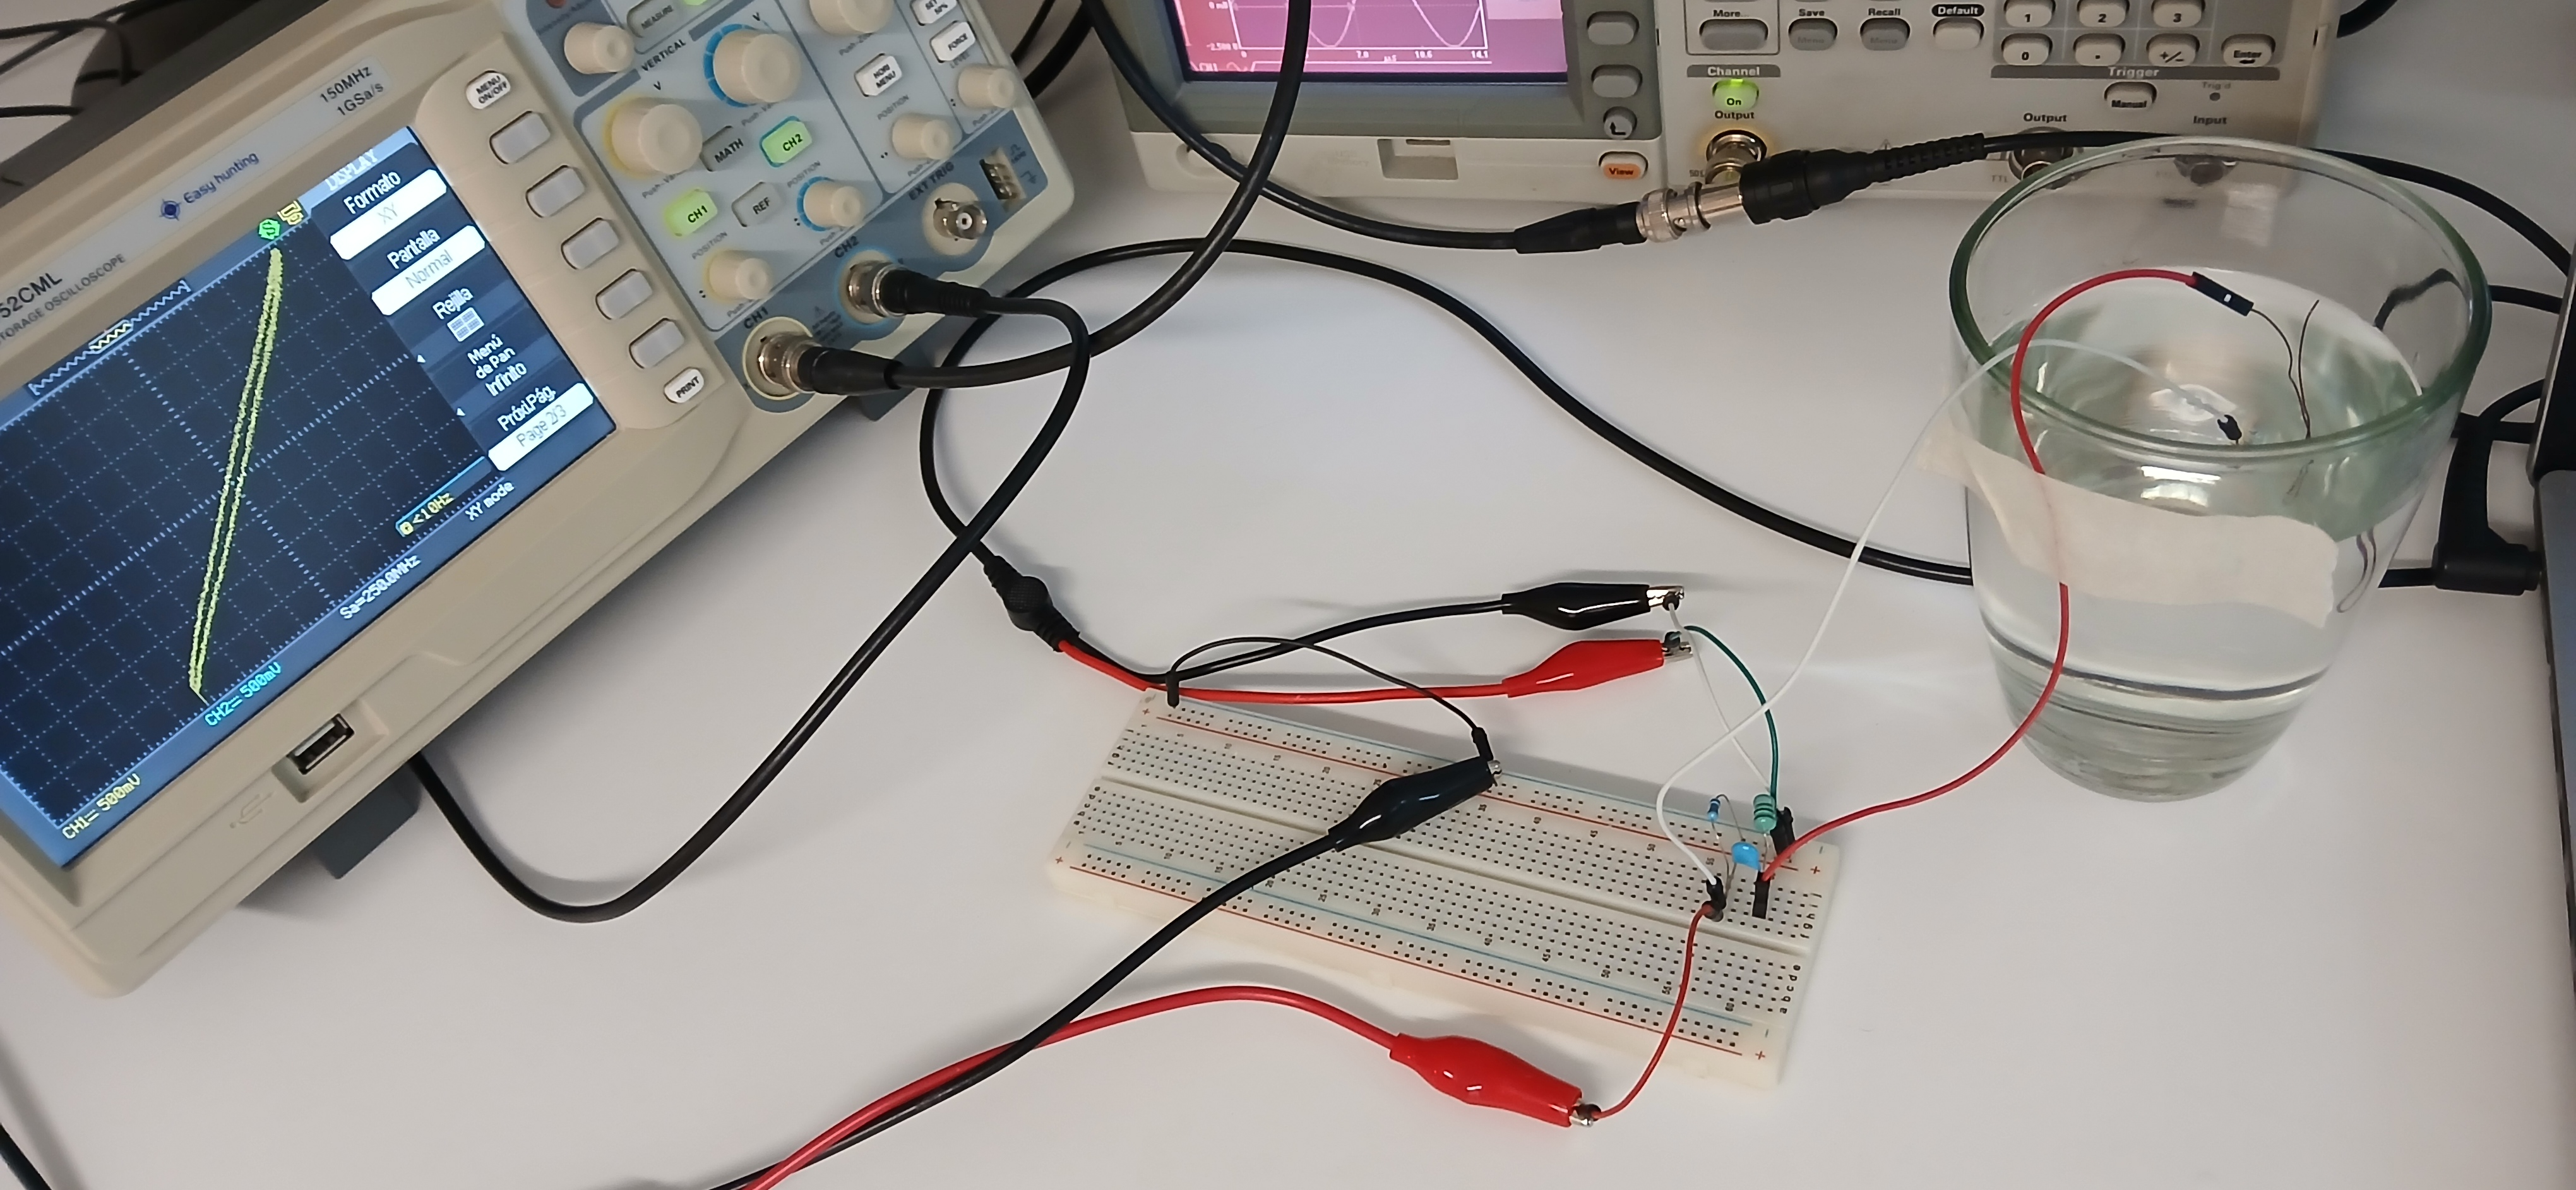
\includegraphics[width=0.7\linewidth]{Figures/05_05_2025/20250507_104355.jpg}
	\caption{Foto del setup para probar lo que pasa al sumergir el alambre de cobre en agua destilada.}
	\label{fig:foto_05_05_2025}
\end{figure}

Ahora voy a cambiar la frecuencia para que esté en resonancia en el aire y después lo voy a sumergir un poco a ver cuánto cambia.
Para evitar que el extremo no esmaltado (donde corté con el alicate) toque el agua y cierra el circuito directamente lo voy a poner doblado, de forma que quede en el aire, y la distancia sumergida sería el doble de la real.

La nueva frecuencia de resonancia es 151.740 kHz. Una cosa \textbf{importante} es que cuando toco el cable con la mano para moverlo cambia la capacitancia y se agrega una fase extra. Con mi mano sobre el cable pin la frecuencia de resonancia da 149.300 kHz. Efectivamente la figura de Lissajeous se abre al tocar el agua (al alambre le cuesta entrar por la capilaridad, pero solo tocarla ya cambia la capacitancia) y pareciera que al sumerjirlo aumenta hasta saturar a cierta profundidad. 


Ahora lo pegué con cinta al vaso para no tener que tocarlo. Ajusto la frecuencia de resonancia a 142.270 kHz. Al moverse el agua cambia la fase, pero es muy sensible. Ahora parece que cambió la frecuencia de resonancia a 142.040 kHz.

Bien, ahora cambió a 142.870 kHz al sumergirlo menos al alambre. Quiero probar poniendo una regla y agregando agua para ver el orden de lo que mide. Con la regla también cambia la capacitancia (por lo menos tocándola con la mano), y el vaso es curvo, con lo cual no hay forma fácil de colocarla. 

Mover mucho el vaso también cambia la frecuencia de resonancia. Ahora está en 143.620 kHz.  

\subsection*{La medición del voltaje}
Nosotros querríamos que el agua esté a tierra, entiendo que por ahí esto soluciona el problema de que acercar cualquier cosa a los cables hace que varía mucho la capacitancia. Sin embargo para poder medir con el osciloscopio la caída de voltaje sobre la resistencia ésta debe estar a Tierra. Se puede medir flotante usando dos canales del osciloscopio y la función math -, pero
no pude camiarle la escala para probarlo y además así no podríamos medir la referencia ya que hay solo dos canales.

Acabo de pensar que si ponemos la Tierra entre la capacitancia y la resistencia por ahí funcionaría bien.



\subsection*{El sensor}
Llevé al taller la pieza impresa que conecta al sensor y tornillo micrométrico al perfil de aluminio para que le corten la T y poder conectarlo al perfil, que Pablo había empezado a sacar el Viernes pasado con un Dremel. 

Lo arrancó con un destornillador largo y lijó un poco con una lija de las cilíndricas de metal y entró perfecto en el tornillo. 

Después de eso monté todo ya con los tornillos correspondientes y pasé los alambres de cable (pelado en una de las puntas) y acero, que verifiqué con el multímetro que no estuviese recubierto de algún tipo de esmalte. Fue complicado engarzar al alambre de acero por los canales del modelo impreso en 3D y no quedó del todo derecho. Todavía faltan las tuercas M4 para terminar de cerrar más fuerte el sensor y por ahí luego si se pueda tirar más fuerte para enderezarlo sin que se salga de los canales. % $ O canaletas.  

Después enrosqué la punta del alambre de cobre al de acero para enderezarlo, corté el excedente del lado enroscado con el alicate y tiré para que quede lo más recto posible. Pero no está demasiado ajustado y se desliza sobre el alambre de acero como si fuese un riel. Quedaría recubrir la punta con el esmalte. Luego si funciona ya quedaría soldar los alambres (que ahora se agarrarían con BNC-pinza-pin a la placa protoboard) al resto de los componentes.


\subsection*{El Arduino} 
Como no pude conectar el osciloscopio a la computadora intenté utilizar el Arduino UNO del Laboratorio para este fin pero tenía muy mala frecuencia de sampleo que no supe cómo subir, costándole incluso medir bien una señal de unos 20 Hz. % a 